\chapter{Case Study}

In this chapter, we will carry out a small reversing engineering task using IDAngr to show a usage example of the tool.

\section{Task description}

The task is reversing a custom hash function in an ELF binary for Linux x86\_64. The name of the binary is sftp \footnote{The reader can download the binary here: \url{https://github.com/andreafioraldi/bsc-thesis/raw/master/case_study/sftp}}, a binary exploitation challenge from Google CTF 2018 \cite{gctf} that requires a password to use the program. 

That password hash is hardcoded and the interesting code is the function at address 0x13F0, called by the main.

The rest of the binary is an in-RAM filesystem with a buggy allocator. The challenge was to exploit that bug but we will discuss only the part related to the password discovery.

The output of the decompiler for the function is the following:

\begin{cpp_code}
signed __int64 sub_13F0()
{
  char *v0; // rbx
  __int64 v1; // rdx
  signed __int64 result; // rax
  int v3; // eax
  int v4; // edx
  char v5; // [rsp+0h] [rbp-28h]
  char v6; // [rsp+1h] [rbp-27h]
  char v7; // [rsp+2h] [rbp-26h]
  char v8; // [rsp+3h] [rbp-25h]
  unsigned __int64 v9; // [rsp+18h] [rbp-10h]

  v9 = __readfsqword(0x28u);
  v0 = &v5;
  __printf_chk(1LL, "The authenticity of host '%s (3.13.3.7)' can't be established.\n", off_208B80);
  puts("ECDSA key fingerprint is SHA256:+d+dnKGLreinYcA8EogcgjSF3yhvEBL+6twxEc04ZPq.");
  __printf_chk(1LL, "Are you sure you want to continue connecting (yes/no)? ", v1);
  if ( !(unsigned int)__isoc99_scanf("%3s", &v5) )
    return 0LL;
  if ( v5 != 'y' )
    return 0LL;
  if ( v6 != 'e' )
    return 0LL;
  if ( v7 != 's' )
    return 0LL;
  if ( v8 )
    return 0LL;
  __printf_chk(1LL, "Warning: Permanently added '%s' (ECDSA) to the list of known hosts.\n", off_208B80);
  __printf_chk(1LL, "%s@%s's password: ", off_208B88);
  if ( !(unsigned int)__isoc99_scanf("%15s", &v5) )
    return 0LL;
  v3 = _IO_getc(stdin);
  LOWORD(v3) = v5;
  if ( !v5 )
    return 0LL;
  v4 = 21527;
  do                                            // hashing
  {
    v3 ^= v4;
    ++v0;
    v4 = 2 * v3;
    LOWORD(v3) = *v0;
  }
  while ( (_BYTE)v3 );
  result = 1LL;
  if ( (_WORD)v4 != -29190 )
    return 0LL;
  return result;
}
\end{cpp_code}


\section{Solution}

To bypass the authentication we will use IDAngr.
We are using IDA Pro on Windows and so we start also a remote AngrDBG server on a Linux machine.

\begin{figure}[H]
  \centering
  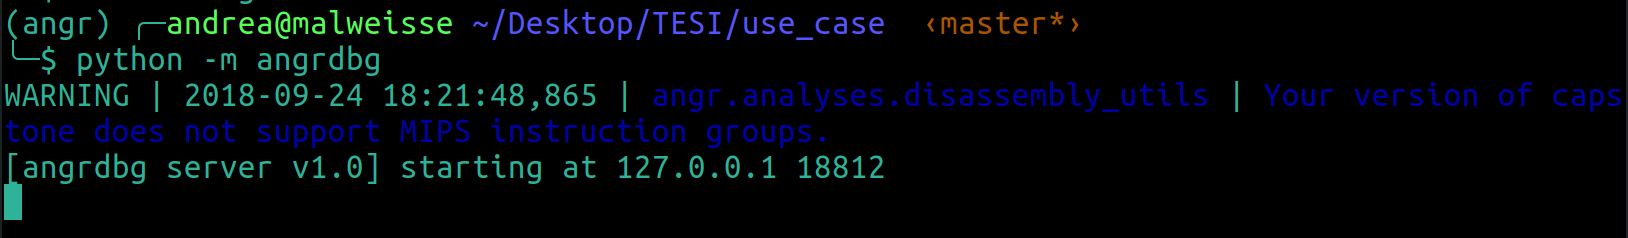
\includegraphics[width=1\textwidth]{u1}
  \label{fig:u1}
\end{figure}

The first step in IDA is to start the debugger and set a breakpoint at line 34 of the function.
This line is just after a scanf call. The inserted string is the password.

As you can see at line 47 the final hash must be -29190, 0x8dfa in hexadecimal.

Running the debugger with F9 the debugged program asks the user to insert the string yes on the standard input.

After that, the program is waiting for the input again using scanf.
Looking at the scanf format \verb|"%15s"| we can know that the password length maximum value is 15, so we insert \verb|aaaaaaaaaaaaaaa| as dummy data.

\begin{figure}[H]
  \centering
  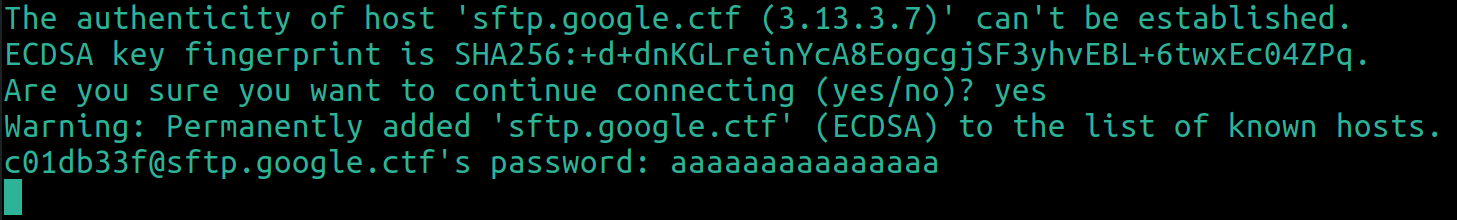
\includegraphics[width=1\textwidth]{u2}
  \label{fig:u2}
\end{figure}

Now the execution has just hit our breakpoint.
At this point, we must invoke the plugin with Ctrl-Alt-I.

The initialization popup asks if we want to use a remote instance of AngrDBG and we insert the correct IP address and port of our Linux machine running the server.

\begin{figure}[H]
  \centering
  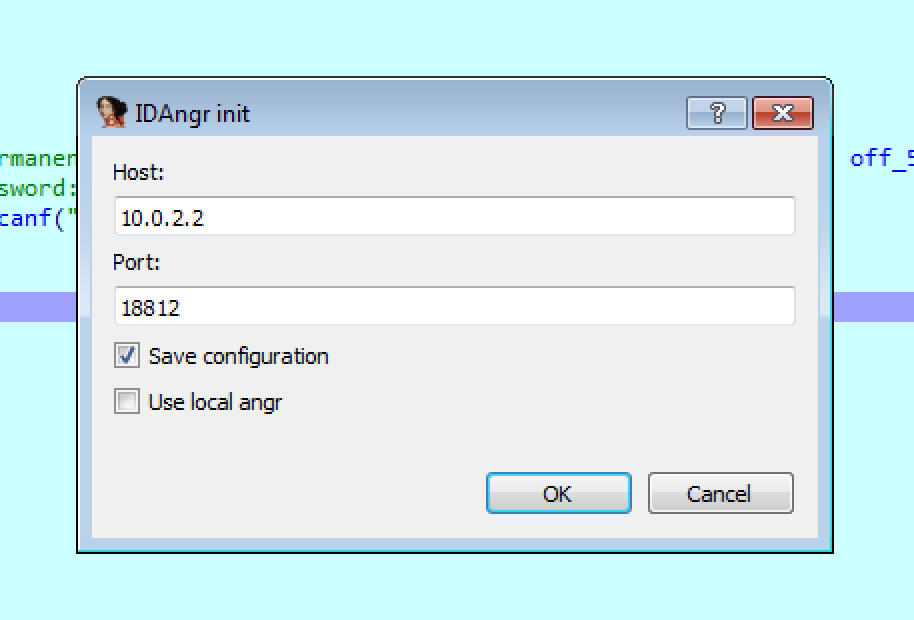
\includegraphics[width=0.6\textwidth]{u3}
  \label{fig:u3}
\end{figure}

Firstly we symbolize the input using the context menu:

\begin{figure}[H]
  \centering
  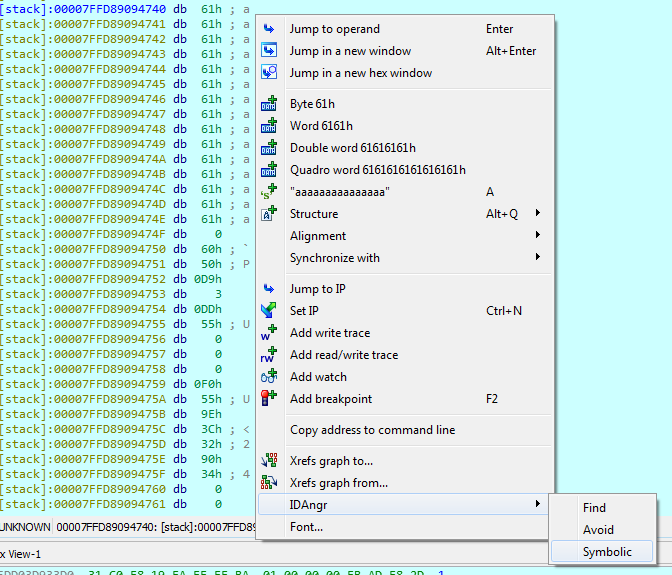
\includegraphics[width=0.6\textwidth]{u4}
  \label{fig:u4}
\end{figure}

In the popup, we set the length of the symbolic value, 15:

\begin{figure}[H]
  \centering
  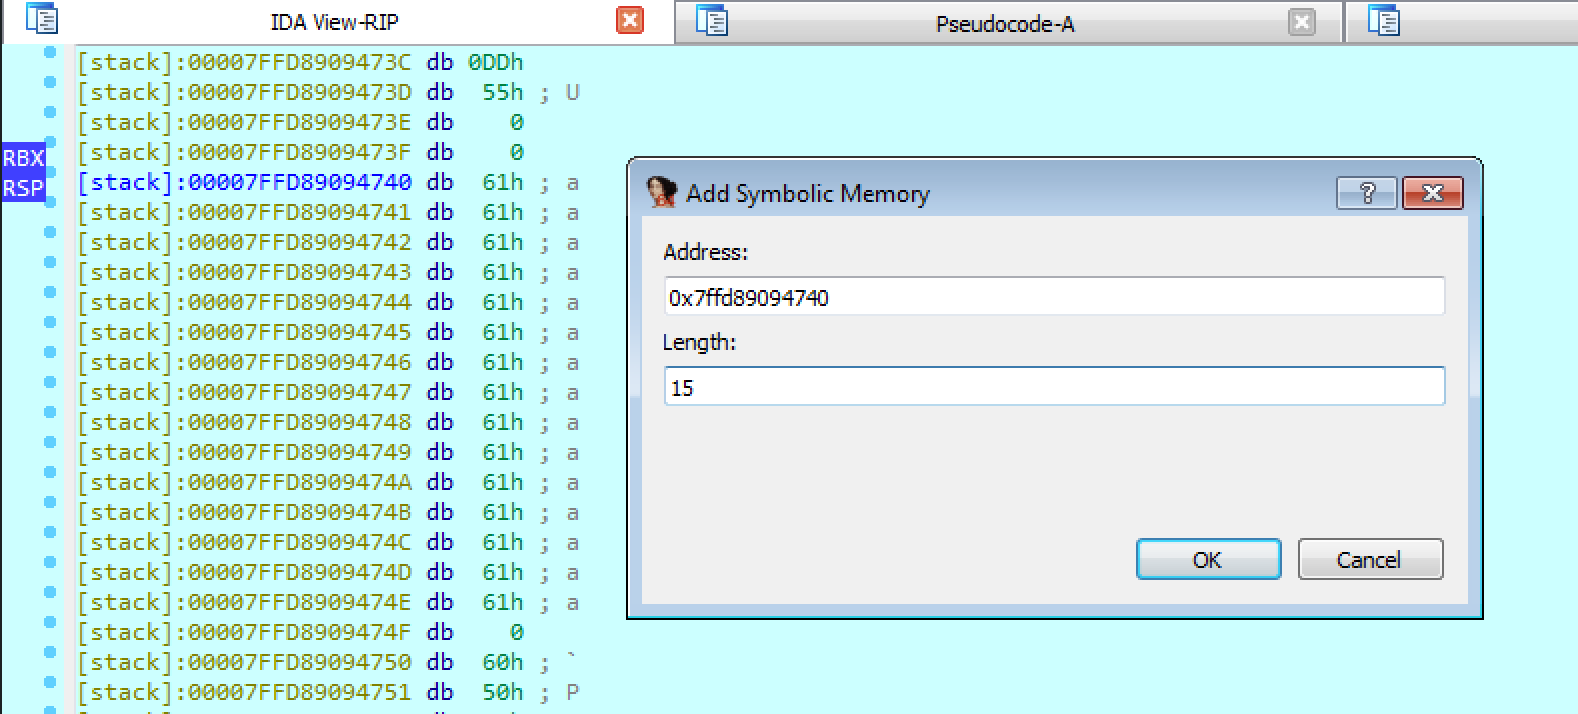
\includegraphics[width=0.8\textwidth]{u5}
  \label{fig:u5}
\end{figure} 

We want also to add pre-constraints to the symbolic input. The password must be composed of printable characters and must not have spaces in order to be compatible with scanf.

By right-clicking on the symbolic value in the panel and selecting \verb|add constraints| we can insert a python snippet and add these constraints:

\begin{figure}[H]
  \centering
  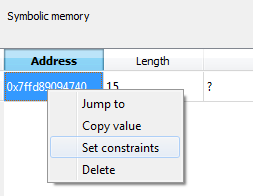
\includegraphics[width=0.4\textwidth]{u6}
  \label{fig:u6}
\end{figure}

\begin{figure}[H]
  \centering
  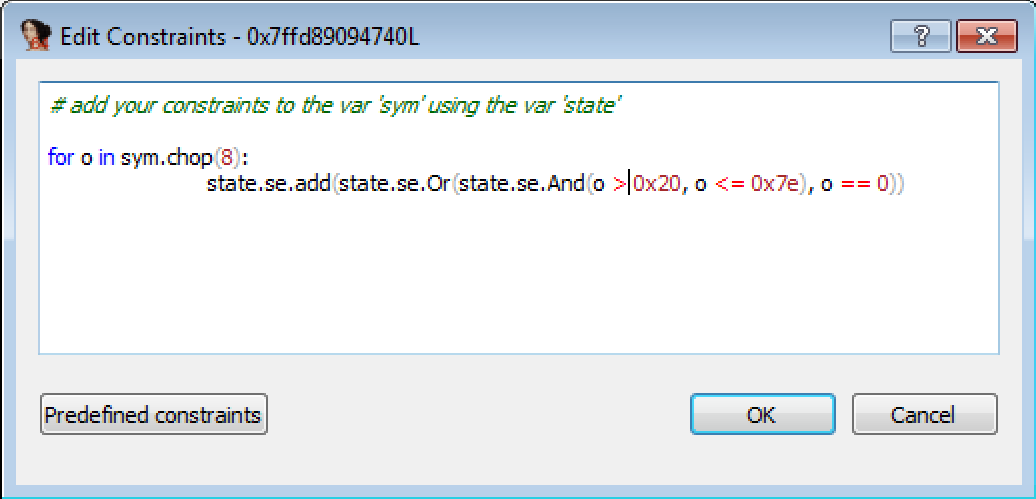
\includegraphics[width=0.8\textwidth]{u7}
  \label{fig:u7}
\end{figure} 

The next step is to select the find and avoid targets. The interesting branch is the hash value comparison at line 47. We want to avoid line 48 and execute line 49. 

In the graph view, the branch is the following. Line 48 is the basic block on the left, line 49 is the block on the right.

\begin{figure}[H]
  \centering
  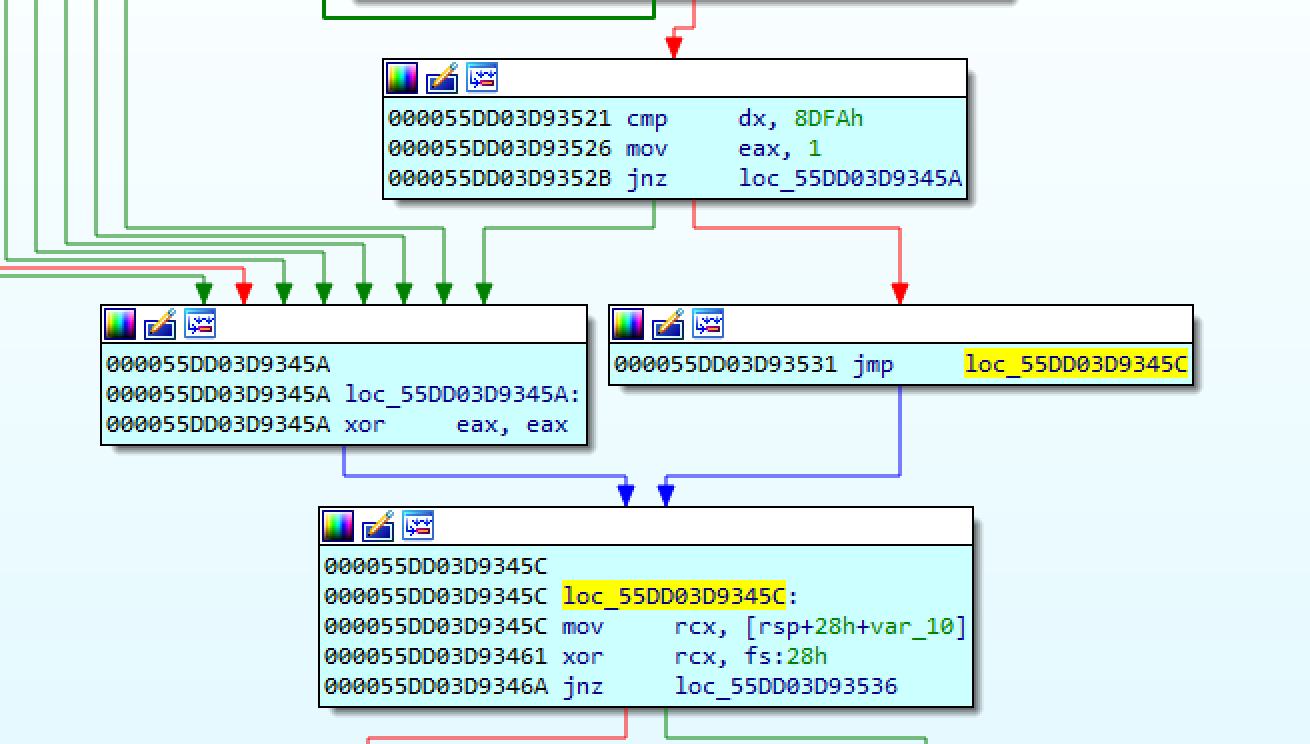
\includegraphics[width=0.8\textwidth]{u8}
  \label{fig:u8}
\end{figure} 

Using the context menu we set the instruction addresses corresponding to the two lines of code as avoid and find targets, respectively:

\begin{figure}[H]
  \centering
  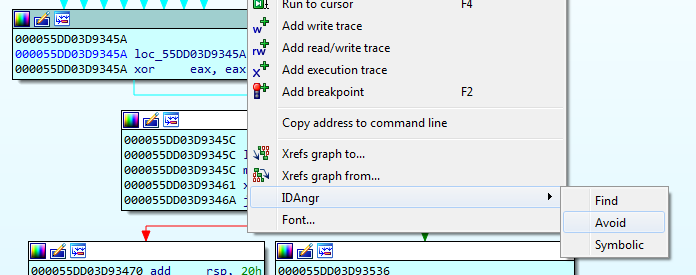
\includegraphics[width=0.8\textwidth]{u9}
  \label{fig:u9}
\end{figure} 

We can now run the exploration clicking on the RUN button to show the exploration prompt. In this prompt we leave as selected the default memory type, \verb|use simprocs in got when possible|. We are not exploring external code so all the memory types have the same behavior.

\begin{figure}[H]
  \centering
  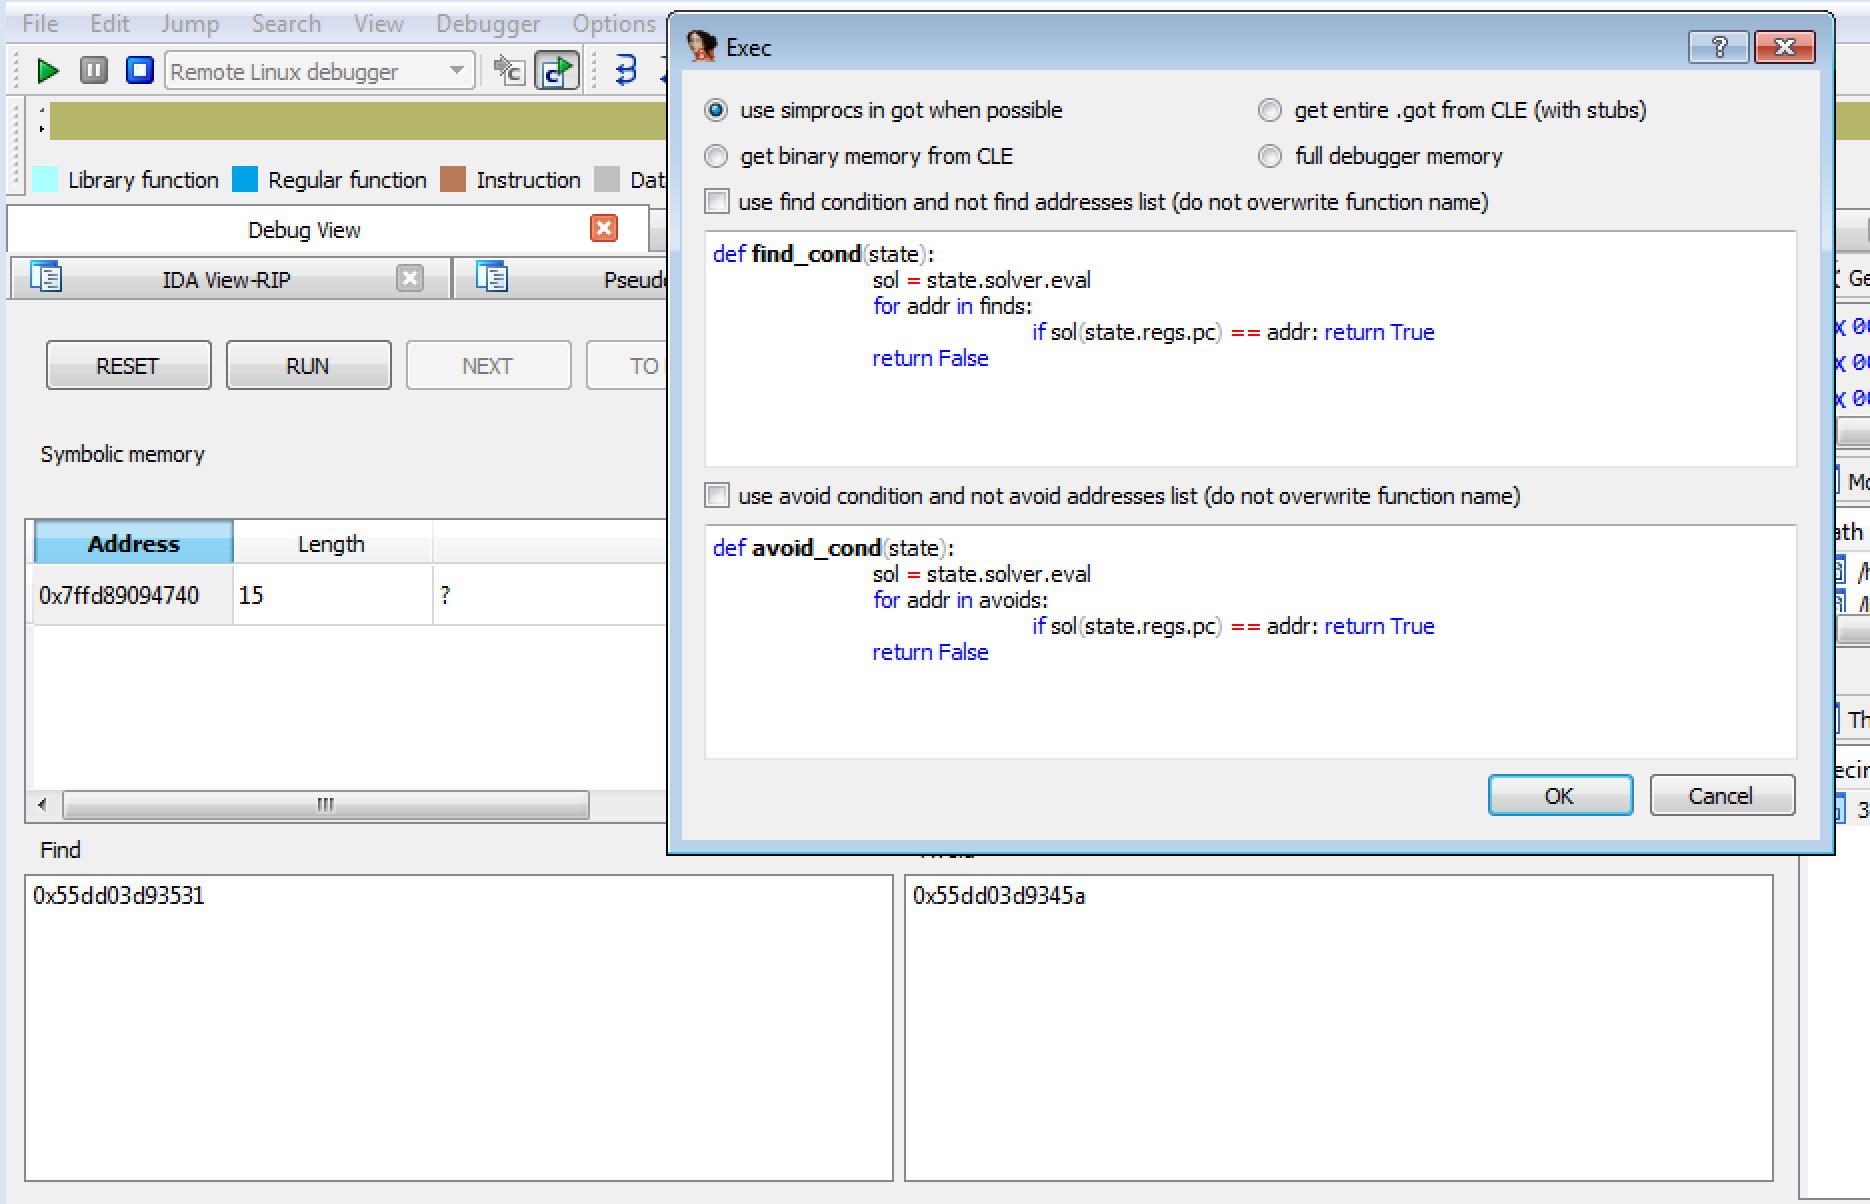
\includegraphics[width=0.9\textwidth]{u10}
  \label{fig:u10}
\end{figure} 

We click on OK to start the exploration.
After some time we get a valid concretized value of the password in the panel. 

\begin{figure}[H]
  \centering
  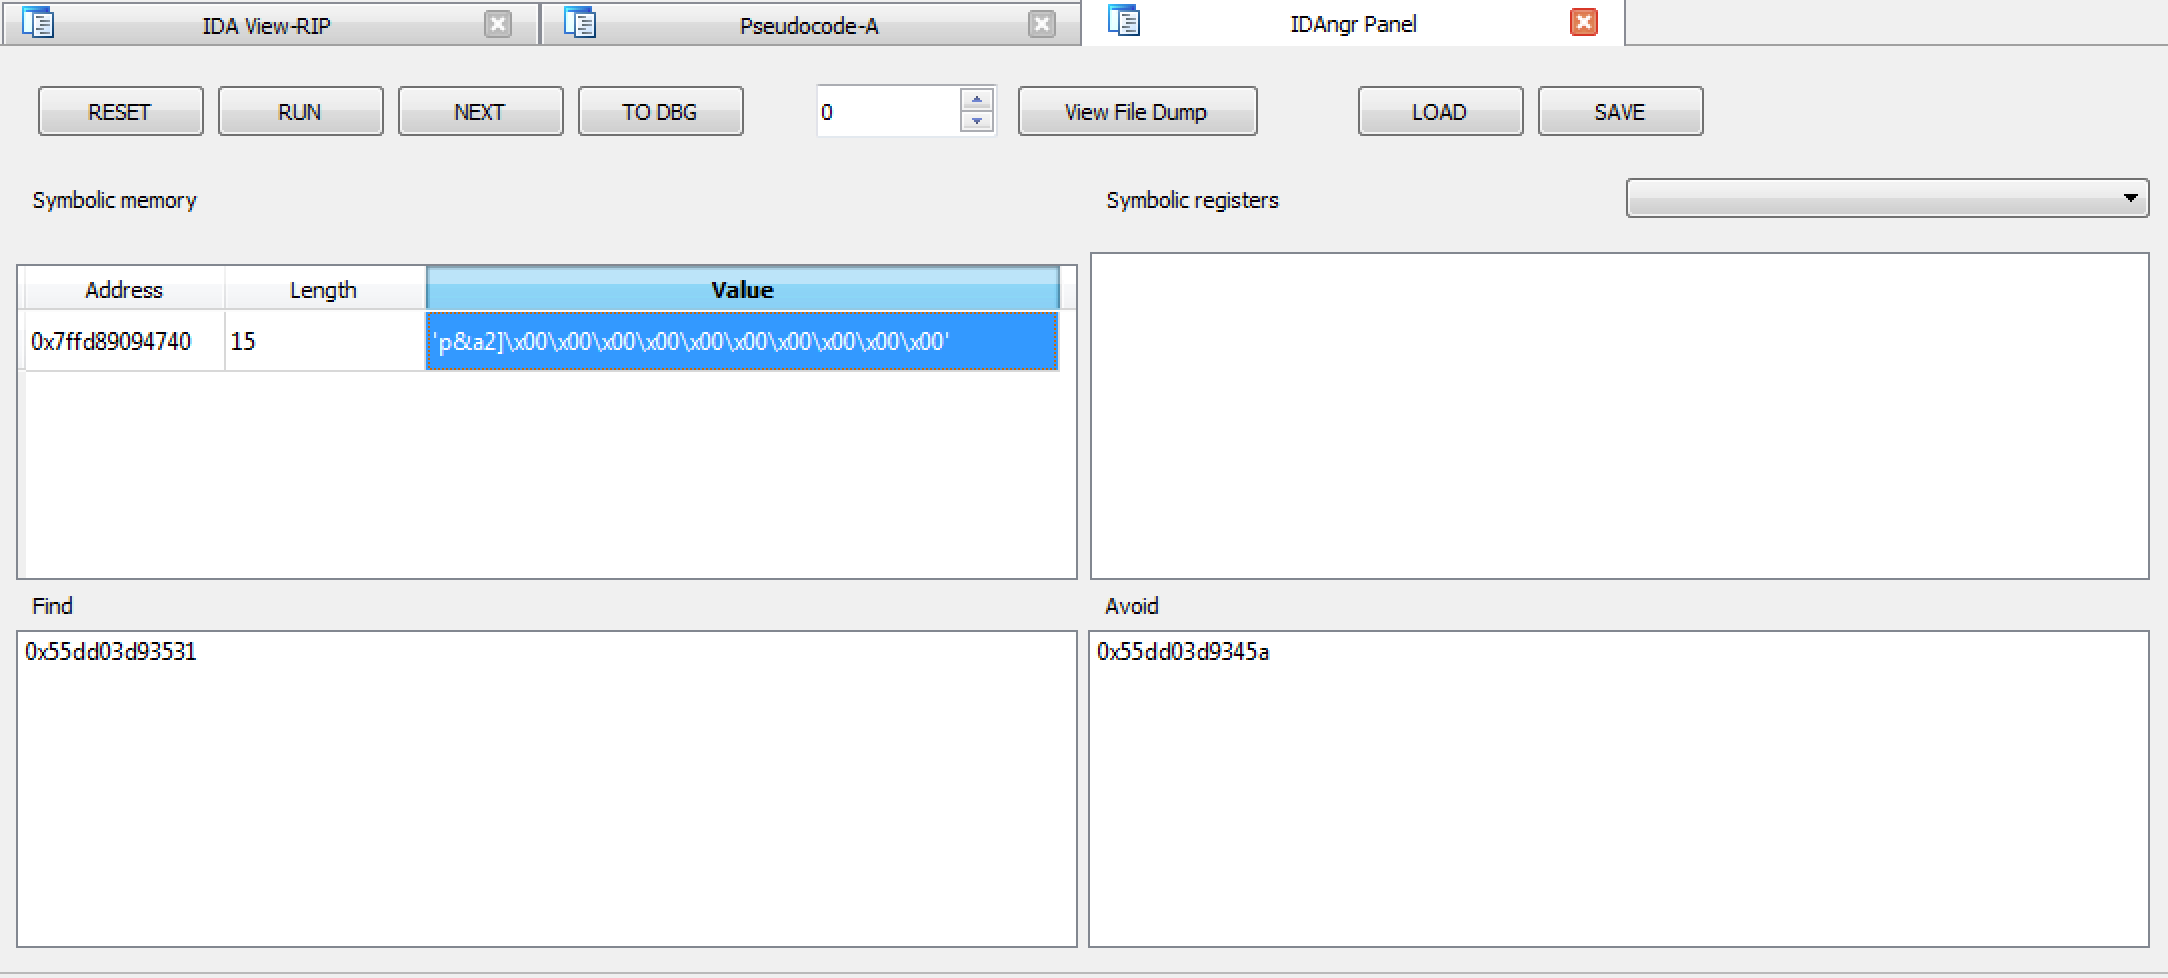
\includegraphics[width=1\textwidth]{u11}
  \label{fig:u11}
\end{figure}

This is our solution. We can now use the "TO DBG" button to inject this value in the debugger memory:

\begin{figure}[H]
  \centering
  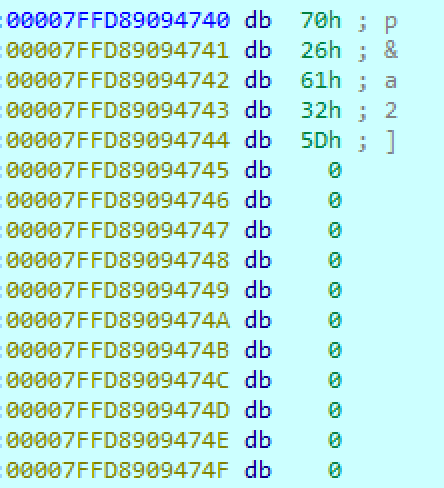
\includegraphics[width=0.4\textwidth]{u12}
  \label{fig:u12}
\end{figure}

By stepping with the debugger until the end of the function we reach line 49 rather than line 48. The authentication is successful.

\begin{figure}[H]
  \centering
  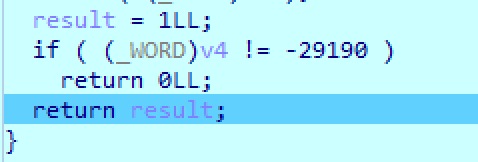
\includegraphics[width=0.4\textwidth]{u13}
  \label{fig:u13}
\end{figure}


\section{Discussion}

This simple use case, in our opinion, shows how user-friendly the IDAngr graphical interface is.
The user interaction is a crucial feature of the technique. Reverse engineering is and will be a manual task and having a comfortable interface make a difference.
Of course, state synchronization is not limited to the exploration of simple pieces of code like the one in the example, but this Google CTF challenge is representative of the workflow that a reverser can carry out assisted by our tool.


